\chapter{RESULTADOS E Discussões}\label{ch:intro}
Utilizando os materiais e métodos previamente apresentados, neste capítulo serão
apresentados e discutidos os resultados obtidos a partir dos experimentos abordados na base de imagens criada, assim como comparações com os efeitos de processamento de imagens aplicados na base de imagens coletada. Os resultados serão apresentados na ordem de imagens classificadas em ambiente de luminosidade favoráveis até as imagens capturadas em ambiente noturno.


As métricas apresentadas foram calculadas obtendo-se uma média de assertividade do resgate correto dos caracteres do nome do medicamento em questão, analisando a quantidade de caracteres e quantidade de resgates corretos.

 No decorrer da criação da base de imagens, foi constatado que o dispositivo celular Samsung J2 utilizado para testes, não possui boa captura de imagens em ambientes com baixa luminosidade e ainda assim, optou-se por continuar com a captura de imagens e os testes, pelo fato de poder reproduzir uma situação real, que pode ocorrer com futuros usuários da aplicação em estudo.
 
Os testes foram realizados e comparados entre as categorias de imagens, perspectivas e entre as técnicas de processamento de imagem. Os testes foram encerrados quando três testes consecutivos da mesma categoria de imagens não obtiveram resgates de pelo menos 3 caracteres corretos e em sequência, denominando que a abordagem do PDI não estava correta, o que impossibilitou o próximo passo, que é a recuperação dos registros na base de dados descritiva dos medicamentos.


Em todos os experimentos que serão apresentados, foi necessário importar as fotos do banco de imagens de cada categoria como forma de \textit{asset}, a fim de minimizar tempo entre os testes. Importar como \textit{asset} é a forma correta onde possibilita a importação de uma imagem em um aplicativo de celular. A base de imagens importada foi excluída após os testes necessários, essa medida foi tomada para otimizar e minimizar o tempo de testes.

Como forma de simplificar posteriormente as buscas na base de informações de remédios, foram ignorados os acentos, o que não impactará nos resultados do OCR demonstrados a seguir. Dessa maneira, caso o OCR identifique alguma letra que possua acento, é realizado um pós processamento no texto para que a consulta seja feita sem acentos e caracteres especiais, visando deixar a busca simplificada e com um poder assertivo maior.

\section{MANIPULAÇÃO DOS DADOS COLETADOS}

Segundo o Portal da \citeonline{PORTALANVISA}, desde o ano 2000 até 05/08/2019, 5.723 medicamentos genéricos foram registrados. Destes, 2.398 registros foram cancelados, restando 3.325 medicamentos genéricos com registros válidos. Em base dessa informação, pensando em trabalhos futuros e pensando em ganho de desempenho no dispositivo celular, foi optado por manipular os dados via \textit{JSON}, viabilizando de forma mais dinâmica o uso de banco de dados não relacionais, chamados de NoSQL, que trabalham diretamente com arquivos JSON.

Os dados coletados para este trabalho foram capturados manualmente do bulário da Anvisa, que disponibiliza documentos digitalizados contendo informações da bula, possibilitando que as informações dos remédio fossem retirados manualmente no formato JSON, para cada medicamento de referência deste trabalho. Foi optado que as informações fossem armazenadas no formato JSON para facilitar a busca detalhada pela lista de objetos criadas do tipo Medicamento, onde possui as seguintes chaves de identificação:

\begin{lstlisting}[firstnumber=1]
{
  "medicamentos": [
      {"id": 1},
      {"nome": "descricao"},
      {"principios_ativos": "descricao"},
      {"contra_indicacoes": "descricao"},
      {"tipo_medicamento": "descricao"},
      {"data": "Descricao"}
    ]
}
\end{lstlisting}
\fonte{Autoria Própia.}


Com retorno obtido do OCR Firebase MLKit, é possível obter os textos em blocos, linhas e palavras, conforme descrito na sessão 2.5.2, possibilitando realizar uma rápida busca no documento \textit{JSON} local. Por este motivo, foi elaborado um processo com 6 algoritmos de pós processamento dos dados, no intuito de efetuar uma busca mais refinada e assertiva dos dados coletados do OCR na base de dados JSON, que são:
 \begin{figure}[h!]
	\centering
	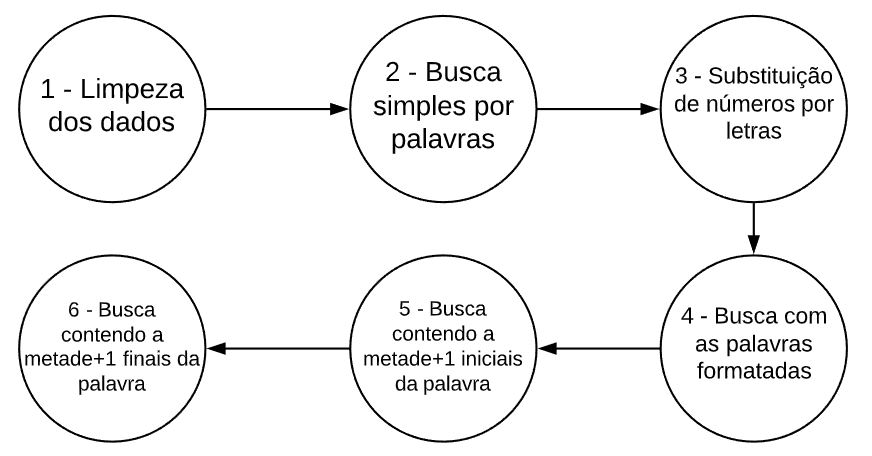
\includegraphics[width=0.99\textwidth]{Imagens/steps.JPG} 
	\caption[Etapas de pós processamento do OCR.]{Etapas de pós processamento do OCR.}
\fonte{Autoria Própria.}
	\label{app}
\end{figure}
\begin{enumerate}
  \item Limpeza dos dados coletados;
  \item Busca simples por palavras;
  \item Substituição de números visualmente similares a letras;
  \item Busca por palavras formatadas;
  \item Busca contendo a metade das letras iniciais das palavras;
  \item Busca contendo a metade das letras finais de cada palavra.
\end{enumerate}

%EVERTON: Você usa muito feito. Feito é fazer, construir. Procure melhorar esta situação no documento.
Na primeira etapa, algumas palavras padrões foram identificadas durante o estudo das caixas de medicamento como por exemplo: ``VENDA SOB PRESCRIÇÃO MÉDICA'', ``50 mg'', ``Uso OraL'', ``Uso adulto'' e ``Contém 20 comprimidos''. Essas palavras serão excluídas neste trabalho, porém elas podem servir de informações adicionais e podem ser relevantes para um sistema mais criterioso em trabalhos futuros.

Supondo que uma caixa de medicamento não contenha mais de 50 palavras, na segunda etapa do processo foi analisado que se faz viável a comparação de todas as palavras encontradas com todos os registros de chave de valor ``nome'' do documento JSON. Mesmo que seja encontrado algum registro, será efetuado a terceira etapa.

Na terceira etapa, é feito um segundo refinamento das informações nas palavras encontradas, se possuir caracteres iguais ao número 0, substituir pela letra ``O'', número 1 pela letra ``L'', número 4 pela letra ``A'' e também o número 7 pela letra ``T'', devido o seu alto grau de semelhança visual para o OCR. 

Após feito a troca dos caracteres, será feita uma nova busca na base de dados JSON, passando palavra por palavra que representa a quarta tarefa da lista. Caso não seja encontrado nenhum registro, o algoritmo % COMO ASSIM?? 
interpretará o quinto passo, que é a separação da palavra ao meio, formando 2 partes, do início da palavra até a metade e da metade até o final, possibilitando a busca novamente na base por medicamentos que contenham essa sequência de letras na chave ``nome'' do documento JSON.

A cada medicamento encontrado nas etapas, o medicamento é inserido em uma lista que por fim será apresentada para o usuário, retornando apenas os medicamentos distintos encontrados. Caso haja mais de um medicamento encontrado na base, será apresentado uma lista simples, para que o usuário selecione o medicamento correto, para então encontrar o conteúdo do medicamento inspecionado em questão, conforme demonstrado na Figura \ref{app}. 

 \begin{figure}[h!]
	\centering
	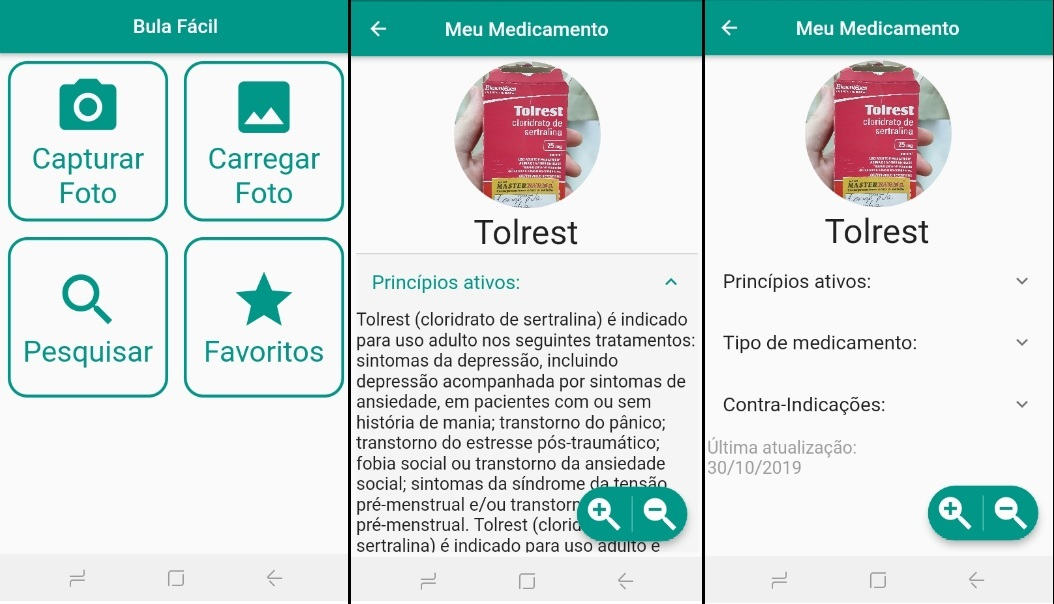
\includegraphics[width=0.99\textwidth]{Imagens/telas_app.jpg} 
	\caption[Resgate e apresentação do medicamento Voltaren.]{Resgate e apresentação do medicamento Voltaren.}
\fonte{Autoria Própria.}
	\label{app}
\end{figure}

\section{Experimento sem manipulação de imagem}
Os resultados apresentados na Tabela \ref{tab:exp_sem_filtro}, são referentes às imagens originais submetidas ao OCR, sem nenhum tipo de tratamento de imagem. As colunas de categorias de imagens são compostas por 30 imagens, e os testes da Tabela \ref{tab:exp_sem_filtro} demonstram o resultado dos experimentos aplicados a todas as categorias. A taxa de acurácia com pós-processamento de dados é de 100\%, alcançando um estado ótimo de reconhecimento do medicamento. 

Foi posível observar uma deficiência grande no OCR ao reconhecer o medicamento Tolrest, que possui no seu nome, a última letra representada pela letra ``L" com uma fonte diferente, como representado na Figura \ref{exemplares}, ocasionando uma pequena deficiência no OCR, representada pela taxa de 83,3\% de acurácia em algumas categorias de imagens, o que se fez necessário a execução dos passos de pós-processamento já citados anteriormente.

O passo de pós-processamento eficiente para este caso foi o passo 5, responsável por efetuar a busca com metade dos caracteres da palavra + 1, encontrando com eficiência o nome correto na base de dados.



\begin{table}[]
\centering
\begin{tabular}{lccccc}
\hline
Procedimentos & set1 & set2 & set3 & set4 & set5 \\ \hline
Tempo da Captura da Imagem & 49 sec & 52 sec & 52 sec & 49 sec & 50 sec \\
Tempo de PDI & 0 sec & 0 sec & 0 sec & 0 sec & 0 sec \\
Tempo do OCR & 22 sec & 34 sec & 27 sec & 25 sec & 32 sec \\
Acurácia OCR & 100\% & 83,3\% & 100\% & 83,3\% & 83,3\% \\
Tempo do pós-processamento & 0 sec & 5 sec & 0 sec & 4 sec & 5 sec \\
Acurácia com pós-processamento & 100\% & 100\% & 100\% & 100\% & 100\% \\
Tempo Total & 72 sec & 91 sec & 80 sec & 78 sec & 87 sec \\ \hline
\end{tabular}
\caption{Experimento sem aplicar PDI. set1: Boa luminosidade, set2: Baixa luminosidade, set3: Ambiente externo, set4: Noturnas sem flash, set5: Noturnas com flash}
\label{tab:exp_sem_filtro}
\fonte{Autoria Própria.}	
	\label{fig:exp_sem_filtro}
\end{table}


\section{EXPERIMENTO APLICANDO efeito DE ESCALAS EM CINZA}

\begin{table}[]
\centering
\begin{tabular}{lccccc}
\hline
Procedimento & set1 & set2 & set3 & set4 & set5 \\ \hline
Tempo da Captura da Imagem & 49 sec & 52 sec & 50 sec & 49 sec & 50 sec \\
Tempo de PDI & 83 sec & 118 sec & 99 sec & 600+ sec & 388 sec \\
Tempo do OCR & 28 sec & 39 sec & 28 sec & - & 40 sec \\
Acurácia OCR & 77\% & 45\% & 77\% & 0\% & 16,6\% \\
Tempo do pós-processamento & 4 sec & 2 sec & 4 sec & - & 1 sec \\
Acurácia com pós-processamento & 100\% & 83,3\% & 100\% & 0\% & 16,6\% \\
Tempo Total & 164 sec & 211 sec & 181 sec & 600+ sec & 474 sec \\ \hline
\end{tabular}

\caption{Experimento aplicando filtro de escalas em cinza. set1: Boa luminosidade, set2: Baixa luminosidade, set3: Ambiente externo, set4: Noturnas sem flash, set5: Noturnas com flash}
	\label{tab:exp_grey_scale}
\fonte{(Autoria Própria)}	

\end{table}
Para aplicar o filtro de imagem em escalas de cinza, foi necessário implementar um algoritmo para tal função. Como a captura de imagem manipula um objeto do tipo \textit{File} (arquivo) da galeria, foi necessário decodificar o \textit{File} e transformar para um objeto do tipo \textit{Image}. 

Para otimizar tempo e recurso de memória do celular que acabou sendo insuficiente, foi necessário fazer uma transformada no tamanho da imagem, para altura igual a 600 e largura igual a 600. Com o array de bits gerado da imagem, foi possível iniciar a conversão da imagem para escala de cinza, deixando assim, a imagem em escala de cinza pronta para ser aplicada ao OCR.


Os resultados do experimento de pré processamento aplicando efeito de escalas em cinza na imagem, são apresentados na Tabela \ref{tab:exp_grey_scale}.






\section{EXPERIMENTO APLICANDO efeito DE Sobel}

Para aplicar o efeito de Sobel na imagem, como proposto na sessão de materiais e métodos, foi necessário implementar um algoritmo para tal função. Também neste caso, como está sendo manipulando um objeto do tipo \textit{File} da galeria, foi necessário decodificar o \textit{File} e transformar para um objeto do tipo \textit{Image}. Para otimizar tempo e recurso de memória, foi necessário fazer uma transformada no tamanho da imagem, para altura igual a 600 e largura igual a 600. Com o array de bits gerado da imagem, foi possível iniciar a conversão da imagem aplicando o filtro de Sobel. Deixando assim, a imagem com filtro de Sobel pronta para ser manipulada pelo OCR. 

\begin{table}[]

\centering
\begin{tabular}{lccccc}
\hline
Procedimento & set1 & set2 & set3 & set4 & set5 \\ \hline
Tempo da Captura da Imagem & 49 sec & 52 sec & 50 sec & 49 sec & 50 sec \\
Tempo de PDI & 375 sec & 489 sec & 434 sec & 600+ sec & 600+ sec \\
Tempo do OCR & 25 sec & 27sec & 28 sec & - & - \\
Acurácia OCR & 0\% & 0\% & 0\% & 0\% & 0\% \\
Tempo do pós-processamento & 2 sec & 1 sec & 2 sec & - & - \\
Acurácia com pós-processamento & 0\% & 0\% & 0\% & 0\% & 0\% \\
Tempo Total & 451 sec & 570 sec & 514 sec & 600+ sec & 600+ \\ \hline
\end{tabular}
\caption{Experimento aplicando filtro de Sobel. set1: Boa luminosidade, set2: Baixa luminosidade, set3: Ambiente externo, set4: Noturnas sem flash, set5: Noturnas com flash}
\label{tab:exp_sobel}
\fonte{(Autoria Própria)}	
\end{table}







Como demonstrado na Tabela \ref{tab:exp_sobel}, houve uma grande complicação para processamento da imagem, tanto para a conversão quanto para o OCR de efetuar a extração dos caracteres nas imagens.

\section{Experimento com diferentes perspectivas}
Uma das propostas iniciais deste trabalho a nível de estudo e de possível melhoria do poder assertivo do OCR, foi a correção de perspectiva da caixa de medicamento. As imagens da base de imagens foram capturadas com pequenas diferenças de perspectivas a fim de simular um ambiente real do cotidiano da população. 

Conforme as tabelas demonstradas acima, o OCR não demonstrou nenhuma variação na sua acurácea, sendo desprezível a leve diferença de perspectiva exposta na base de imagens utilizada para testes.

Em testes com uma perspectiva mais agressiva, como por exemplo demonstrado na Imagem \ref{fig:rotacionadas}, foi possível perceber que mesmo com a caixa de medicamento rotacionada aproximadamente 45 graus em relação ao eixo horizontal da base, o OCR foi capaz de reconhecer os caracteres do nome. Já em testes feitos com rotação superior a 50 graus em relação ao eixo horizontal da base, o OCR não obteve retorno de reconhecimento de caracteres. 

É possível afirmar que embalagens de medicamentos podem conter nomes na vertical da base, como por exemplo na Figura \ref{fig:vertical}. Em base dessa afirmação, é necessário realizar um procedimento para a correção de perspectiva rotacionando a imagem capturada em 90º 3 vezes, o que permite obter o reconhecimento do OCR em uma amplitude de 360º em relação ao eixo central do medicamento.

 \begin{figure}[h!]
	\centering
	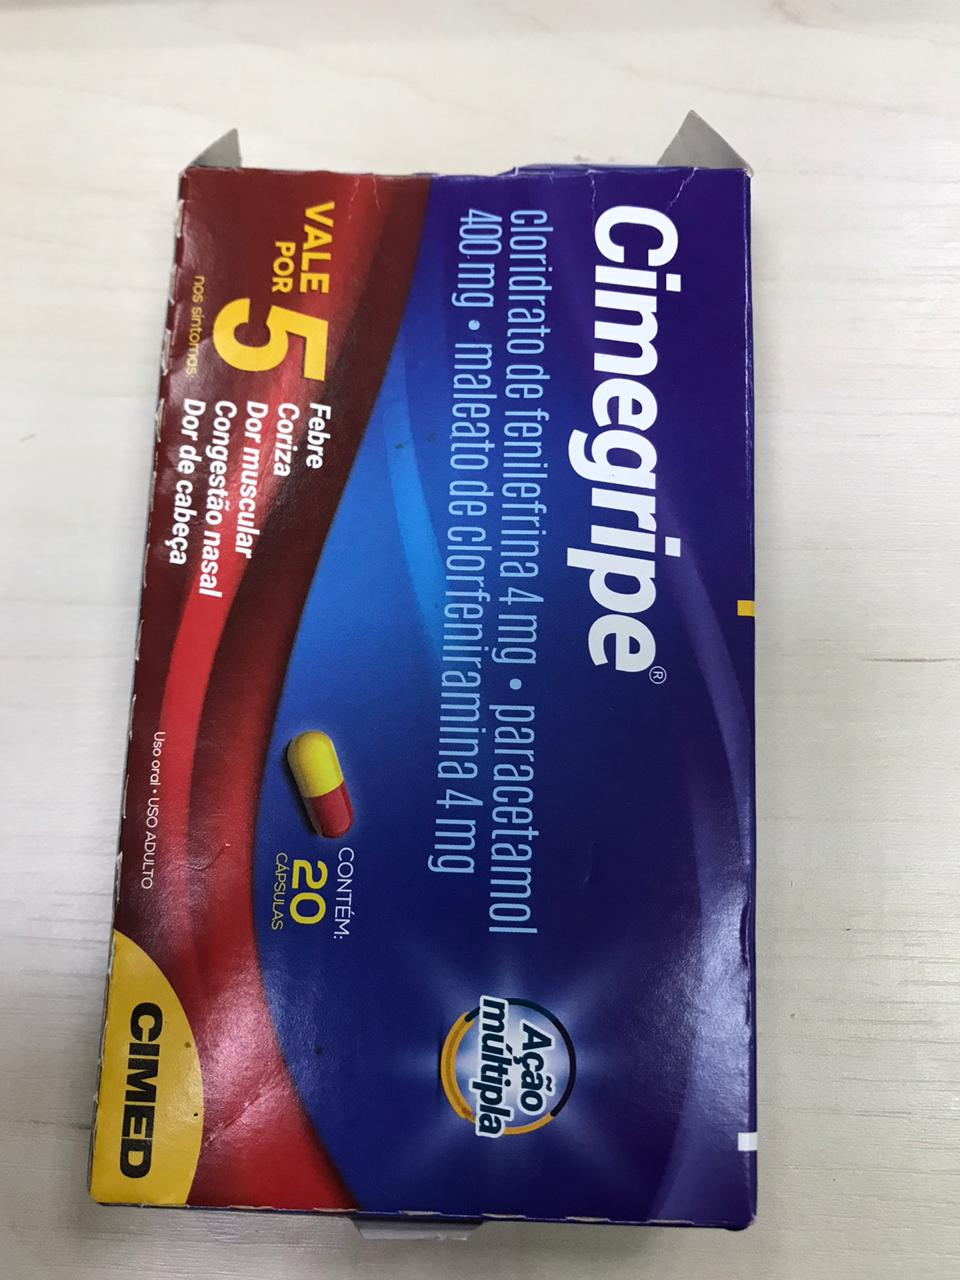
\includegraphics[width=0.4\textwidth]{Imagens/vertical.jpeg} % <- formatos PNG, JPG e PDF
	\caption[Informações na perspectiva vertical.]{Informações na perspectiva vertical.}
\fonte{Autoria Própria.}%citaç\~ao do livro onde pegou a figura	
	\label{fig:vertical}
\end{figure}



 \begin{figure}[h]
	\centering
	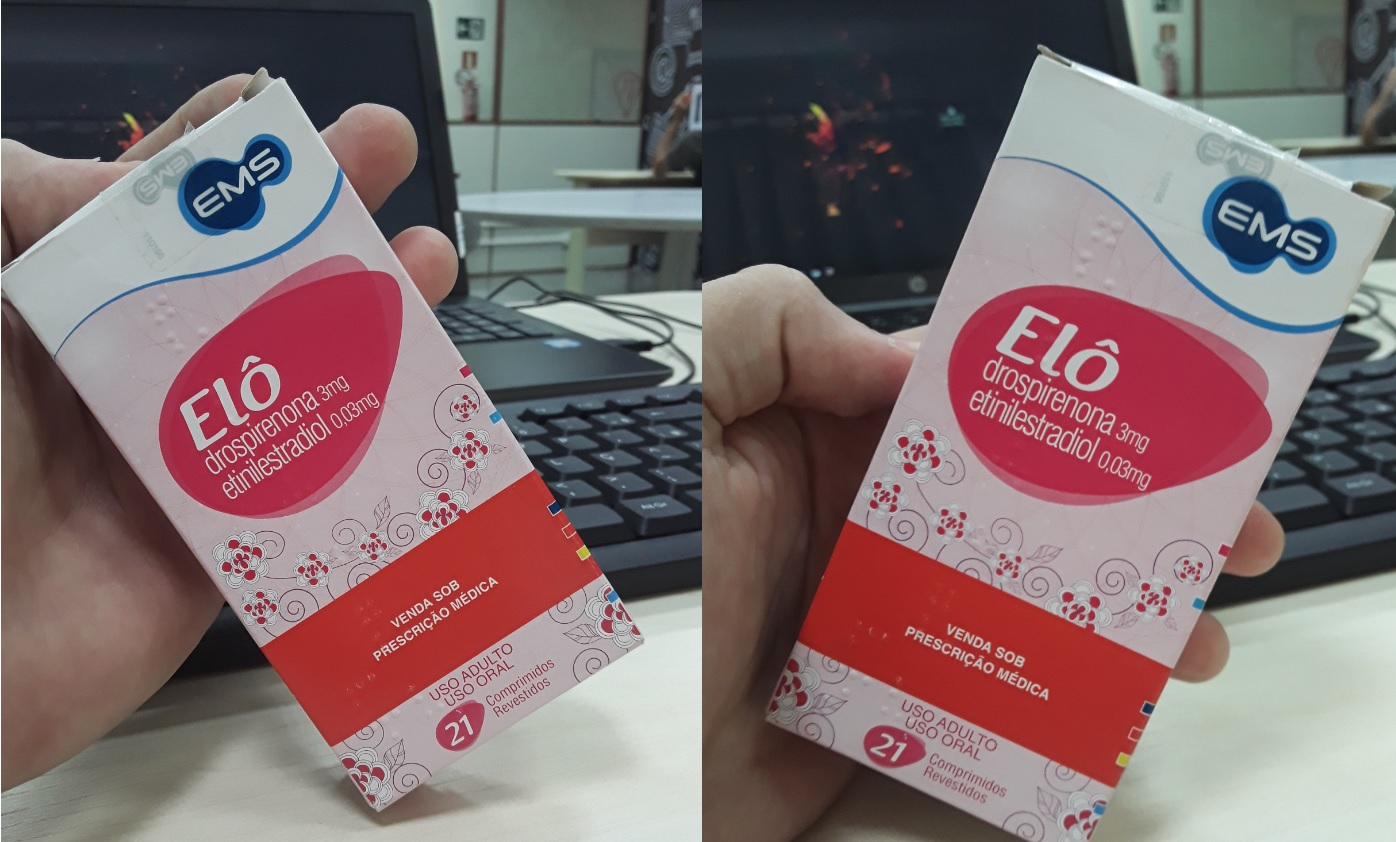
\includegraphics[width=0.6\textwidth]{Imagens/perspectiva2.jpg} % <- formatos PNG, JPG e PDF
	\caption[Imagens rotacionadas.]{Imagens rotacionadas.}
\fonte{Autoria Própria.}%citaç\~ao do livro onde pegou a figura	
	\label{fig:rotacionadas}
\end{figure}

\chapter{CONSIDERAÇÕES FINAIS}\label{ch:intro}
Neste capítulo são resumidas as principais considerações finais acerca do trabalho, bem como suas contribuições sociais. Também são abordados possíveis trabalhos futuros para melhorar e dar continuidade ao objetivo de utilizar técnicas de processamento de imagem juntamente com OCR no auxílio de uma classe social de idosos que vem crescendo continuamente no Brasil.


\section{CONCLUSÃO}

Este trabalho mostrou que é possível desenvolver técnicas de reconhecimento de caracteres em um ambiente \textit{offline} acopladas a aplicativos, sendo possível auxiliar a população no processo medicamentoso. Com uma foto de boa qualidade, luminosidade e resolução maior que 5mp, é possível extrair os caracteres da embalagem do medicamento em questão em pouco menos de 3 segundos, dando um amplo acesso a possibilidades para se trabalhar com esse tipo de dado e solucionando problemas sociais e empresariais.

Com o estudo implementado neste trabalho, é possível levar informação a uma grande parcela da população brasileira que por vezes não dispõe de capacidades visuais para ler letras miúdas de uma bula, pessoas não analfabetizadas, pessoas sem acesso a internet e até mesmo um aplicativo de auto ajuda para o dia a dia de agentes da saúde, que muitas vezes se encontram em locais remotos sem acesso a informações.  

Os testes realizados por meio de um dispositivo físico Samsung J2 com processador de 1.4GHz, equipado com câmera traseira com resolução de 8.0 MP, lançado em outubro de 2015, um celular relativamente antigo e com recursos de memória e processamento limitados (se comparados com celulares lançados em 2019, ano do desenvolvimento do presente trabalho), apresentou dificuldades para efetuar técnicas de processamento de imagens. Os testes aplicando processamento de imagens, em alguns casos causou uma demora de resposta superior a 20 segundos para uma mesma imagem e proporcionando uma acurácia inferior aos testes com imagens sem técnicas de processamento de imagem.

No conjunto de imagens expostas à técnicas de processamento de imagem, as imagens com pré processamento obtiveram menores taxas acurácia e um tempo maior de processamento, uma vez que os recursos de processamento do aparelho celular demonstraram limitados para essa função. Por estes motivos, foi possível observar que o OCR da Google acabou sendo melhor em fotos de uso real do dia a dia e com inclinação de 45 graus em relação a base da lente da câmera.

Os testes realizados foram efetuados com caixas de medicamentos aleatórios, diferentes tamanhos, perspectivas, cores e tonalidades de contraste, o que não foi um grande desafio para o tema proposto. 

Visando trabalhos futuros com consultas de bases de dados mais complexas e externas do celular, foi implementado a regra de estrutura de dados manipulando JSON, onde os dados serão muito melhor trafegados pela rede. Outro lado positivo estudado neste trabalho, foi o OCR do Firebase MLKIT, que apresentou um resultado excelente no resgate de caracteres, chegando quase a perfeição do reconhecimento dos caracteres a nível de nome do medicamento.

\section{trabalhos futuros}


Para possíveis trabalhos futuros baseados neste, se indica:

\begin{enumerate}
\item Ampliar a base de dados descritivas de medicamentos.

  \item Melhorar o algoritmo de busca em lista para ter uma melhor eficácia na identificação do medicamento, caso o OCR venha errar sequência de 3 letras ou mais da palavra do medicamento em questão.
  \item Generalizar o tema proposto, sendo possível trabalhar com diferentes problemas sociais e empresariais.
  \item Criar uma base de dados externa para consultas complexas que possibilite retornar mais informações do medicamento em questão ou até mesmo para apresentar informações mais pertinentes, assim como cadastro de medicamentos não regulamentados pela Anvisa na base de dados descritiva dos medicamentos.
  \item Criar uma rota \textit{online} que possibilite a sincronização da base JSON dos medicamentos reconhecidos pela ANVISA.
\end{enumerate}


